\documentclass[../../main.tex]{subfiles}
\begin{document}

{\bf [解答]}

\begin{figure}[htb]
  \centering
  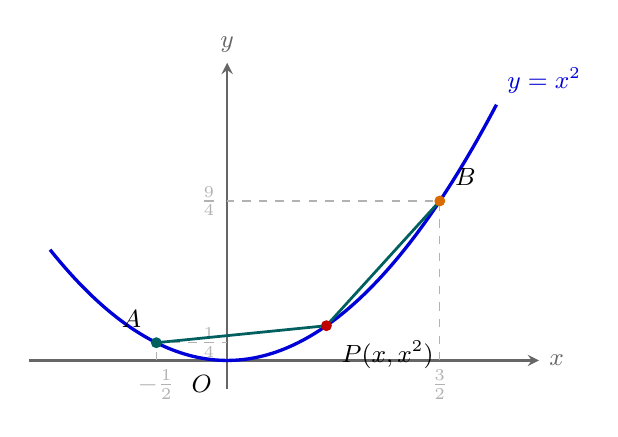
\begin{tikzpicture}[x=1.8cm, y=0.9cm, >=stealth,
    every node/.style={font=\small}]
    \coordinate (O) at (0, 0);
    \coordinate (A) at (-0.5, 0.25);
    \coordinate (B) at (1.5, 2.25);
    \coordinate (P) at (0.7, 0.49);

    \draw[->, thick, gray!80!black] (-1.4, 0) -- (2.2, 0) node[right] {$x$};
    \draw[->, thick, gray!80!black] (0, -0.4) -- (0, 4.2) node[above] {$y$};
    \node[below left=2pt] at (O) {$O$};

    \draw[line width=1.2pt, blue!85!black, domain=-1.25:1.9, samples=80, smooth]
    plot (\x, {\x*\x}) node[above right] {$y=x^2$};

    \draw[dashed, gray!60] (-0.5, 0) node[below] {$-\frac{1}{2}$} -- (A) -- (0, 0.25) node[left] {$\frac{1}{4}$};
    \draw[dashed, gray!60] (1.5, 0) node[below] {$\frac{3}{2}$} -- (B) -- (0, 2.25) node[left] {$\frac{9}{4}$};

    \draw[line width=1.0pt, teal!75!black] (P) -- (A);
    \draw[line width=1.0pt, teal!75!black] (P) -- (B);

    \node[circle, fill=teal!75!black, inner sep=1.4pt] at (A) {};
    \node[circle, fill=orange!85!black, inner sep=1.4pt] at (B) {};
    \node[circle, fill=red!75!black, inner sep=1.4pt] at (P) {};

    \node[above left=2pt] at (A) {$A$};
    \node[above right=2pt] at (B) {$B$};
    \node[below right=2pt] at (P) {$P(x,x^2)$};
  \end{tikzpicture}
  \caption{放物線 $y=x^2$ と2点 $A, B$ および動点 $P$}
  \label{fig:1968_5_parabola_setup}
\end{figure}

$A\left(-\dfrac{1}{2}, \dfrac{1}{4}\right)$, $B\left(\dfrac{3}{2}, \dfrac{9}{4}\right)$, $P(x, x^2)$, $f(x) = |PA|^2 + |PB|^2$ とおく.$f(x)$の関数の詳細を調べれば良い．具体的に計算すると
\begin{align}
  f(x)
  & = \left(x + \dfrac{1}{2}\right)^2 + \left(x^2 - \dfrac{1}{4}\right)^2 + \left(x - \dfrac{3}{2}\right)^2 + \left(x^2 - \dfrac{9}{4}\right)^2 \\
  & = 2x^4 - 3x^2 - 2x + \dfrac{61}{8} \label{eq:1}
\end{align}
だから，一階・2階微分は
\begin{align}
  \begin{cases}
    f'(x) = 8x^3 - 6x - 2 \\
    f''(x) = 24x^2 - 6 = 6(2x+1)(2x-1)
  \end{cases}
\end{align}
である．よって増減表は以下のようになる．

\begin{table}[htb]
  \centering
  \caption{$f(x)$ の増減・凹凸表}
  \label{tab:1968_5_variation}
  \renewcommand{\arraystretch}{1.4}
  \begin{tabular}{c|c|c|c|c|c|c|c}
    \hline
    $x$ & $\dots$ & $-\dfrac{1}{2}$ & $\dots$ & $\dfrac{1}{2}$ & $\dots$ & $1$ & $\dots$ \\ \hline
    $f'(x)$ & $-$ & $-$ & $-$ & $-$ & $-$ & $0$ & $+$ \\ \hline
    $f''(x)$ & $+$ & $0$ & $-$ & $0$ & $+$ & $+$ & $+$ \\ \hline
    $f(x)$ & \carrowDecreaseConvex & $8$ & \carrowDecreaseConcave & $6$ & \carrowDecreaseConvex & 極小 $\dfrac{37}{8}$ & \carrowIncreaseConvex \\ \hline
  \end{tabular}
\end{table}

グラフは下図である．

\begin{figure}[htb]
  \centering
  \begin{tikzpicture}[x=2.7cm, y=0.55cm, >=stealth,
      axis/.style={gray!65, thin},
      guide/.style={gray!55, dashed, thin},
    curve/.style={blue!75!black, very thick}]
    \coordinate (O) at (0,0);
    \coordinate (Ileft) at (-0.5,8);
    \coordinate (Iright) at (0.5,6);
    \coordinate (M) at (1,4.625);
    \coordinate (Yint) at (0,7.625);

    \draw[axis, ->] (-1.13,0) -- (1.55,0) node[right] {$x$};
    \draw[axis, ->] (0,-0.35) -- (0,9.65) node[above] {$y$};
    \node[below left] at (O) {$O$};

    \draw[guide] (Ileft) -- (-0.5,0);
    \draw[guide] (Ileft) -- (0,8);
    \draw[guide] (Iright) -- (0.5,0);
    \draw[guide] (Iright) -- (0,6);
    \draw[guide] (M) -- (1,0);
    \draw[guide] (M) -- (0,4.625);
    \draw[curve, domain=-1.05:1.45, samples=140, smooth]
    plot (\x, {2*(\x)^4-3*(\x)^2-2*(\x)+61/8});

    \node[circle, fill=teal!75!black, inner sep=1.4pt] at (Ileft) {};
    \node[circle, fill=orange!85!black, inner sep=1.4pt] at (Iright) {};
    \node[circle, fill=red!75!black, inner sep=1.5pt] at (M) {};
    \node[circle, fill=blue!75!black, inner sep=1.2pt] at (Yint) {};

    \node[below] at (-0.5,0) {$-\frac{1}{2}$};
    \node[below] at (0.5,0) {$\frac{1}{2}$};
    \node[below] at (1,0) {$1$};
    \node[left] at (0,8) {$8$};
    \node[left] at (0,6) {$6$};
    \node[left] at (0,4.625) {$\frac{37}{8}$};
    \node[above right] at (Yint) {$\frac{61}{8}$};
  \end{tikzpicture}
  \caption{$f(x)=2x^4-3x^2-2x+\dfrac{61}{8}$ のグラフ．変曲点と極小点を示す．}
  \label{fig:1968_5_function_graph}
\end{figure}

従って求める極値と変曲点は以下のようになる．
\begin{itemize}
  \item 極値: $\dfrac{37}{8}$
  \item 変曲点: $\left(-\dfrac{1}{2}, 8\right)$, $\left(\dfrac{1}{2}, 6\right)$
\end{itemize}
凹凸は$x \le \dfrac{-1}{2},\dfrac{1}{2}\le x$では下に凸，それ以外の区間では上に凸である．

\newpage

\end{document}
